%===================================== CHAP 4 =================================

\chapter{Implementation and Datasets}

This chapter covers how the cloud detection framework implemented in this project works, and why it is implemented the way it is. It also covers datasets relevant to this project. For a more thorough walkthrough of how to use the cloud detection framework, see the Appendix. A user manual can also be found in the GitHub repository for this project\footnote{https://github.com/simenvg/cloud\_detection\_framework}. 

\section{Datasets}
The object detection algorithms used in this report all comes with the possibility to train on pre-trained weights. This means that the network has been trained on a dataset and thus already has learned to find features in images and classify them. This is helpful even if the object one wishes to train the algorithm for, is not within the dataset used for finding the pre-trained weights. Using pre-trained weights during training saves computational time for training, and it reduces the required number of training images of the object the detector will be trained on.

\vspace{3mm}

\subsection{Datasets used for pre-trained weights}
The detection algorithms used in this project comes with several different pre-trained weights, where the differences include both network configuration and datasets used in training. The datasets presented here are some of the most common datasets used in object detection and are also used in the training of the pre-trained weights for both Yolo and SSD.


\subsubsection{ImageNet}
ImageNet is a "large-scale ontology of images" \citep{Deng2009}. When \citep{Deng2009} was released in 2009 it stated that the goal of ImageNet was to populate 80,000 subsets of images with 500 to 1,000 pictures. The ImageNet dataset is structured into subtrees and subsets, in an IS A relationship, meaning that if class A is a subset of class B, any object that satisfies class A's specification also satisfies class B's specification. For instance would fish be a subset of an animal. ImageNet contains more than 14 million images that have been annotated by ImageNet with the objects that are in the images. In more than one million of the images bounding boxes are also provided. 


\subsubsection{Pascal, VOC2007 and VOC2012}
Pascal delivers the datasets for the annual Visual Object Classes (VOC) Challenge. The datasets relevant for this report are VOC2007 and VOC2012. VOC2007 consists of 5,011 images with 12,608 objects in the training and validation set, while VOC2012 consists of  11,540 images with 27,540 objects. In figure \ref{fig:VOC2007} and \ref{fig:VOC2012} an overview of classes, images, and objects in VOC2007 and VOC2012 can be found. The combination of these two is denoted as VOC0712.


\begin{figure}[h!]
    \centering
    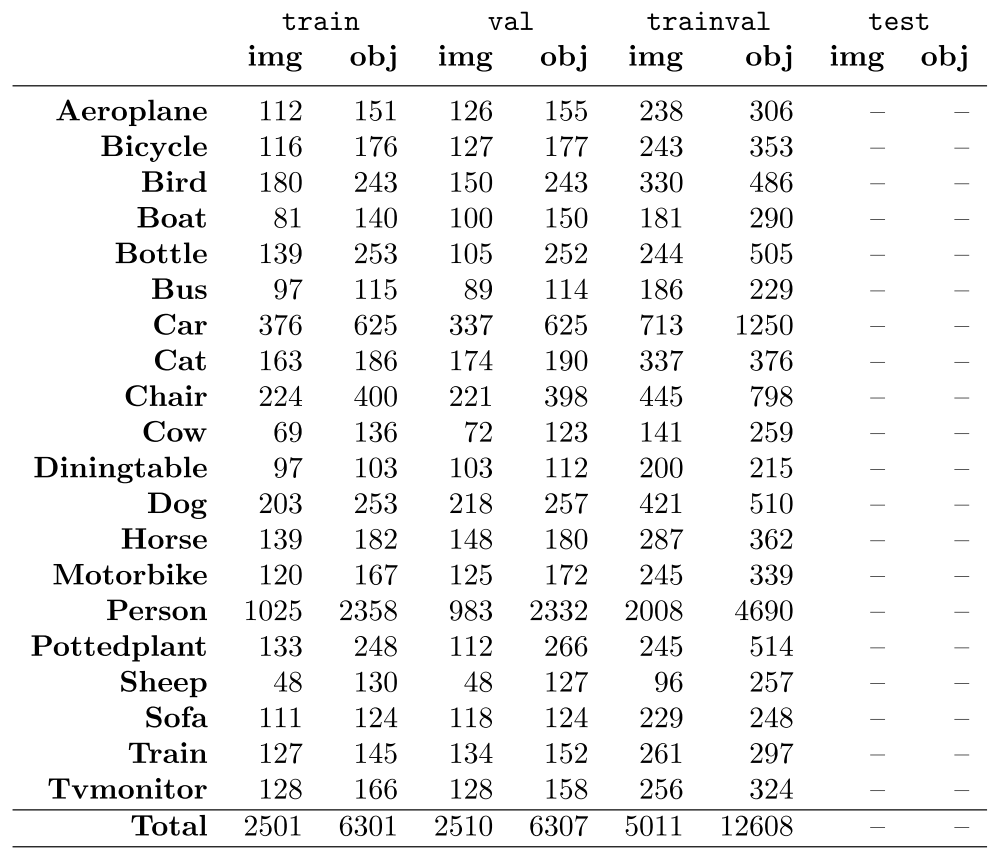
\includegraphics[width=0.55 \textwidth]{fig/VOC2007.png}
    \caption{VOC2007 classes and images, image from \citep{Everingham2007}.}
    \label{fig:VOC2007}
\end{figure}

\begin{figure}[h!]
    \centering
    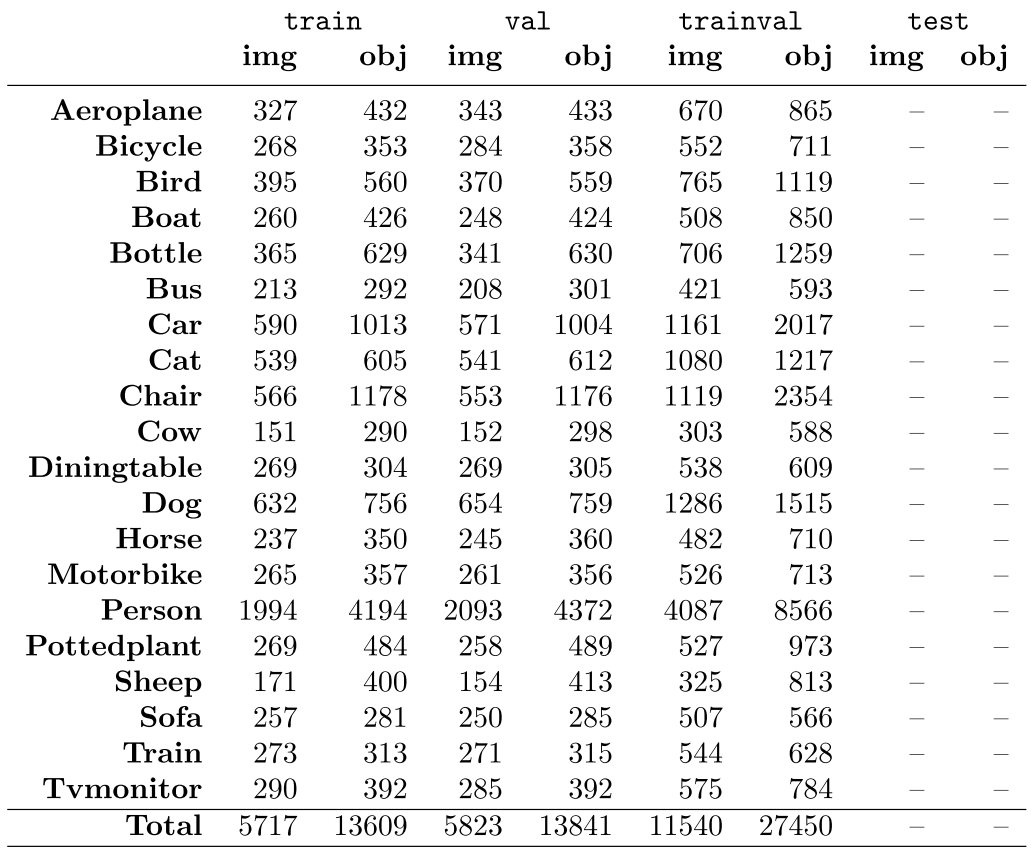
\includegraphics[width=0.55 \textwidth]{fig/VOC2012.png}
    \caption{VOC2012 classes and images, image from \citep{Everingham2012}.}
    \label{fig:VOC2012}
\end{figure}

\clearpage

\subsubsection{COCO}
In 2015 Microsoft released the COCO (Common Objects in Context) dataset \citep{Lin2014}, used for object recognition. The COCO dataset consists of 2.5 million labeled instances in 328,000 images, and are "images of complex everyday scenes containing common objects in their natural context" \citep{Lin2014}. Each object in the image is segmented and labeled separately, instead of semantically which is done in many other datasets. This means that objects of the same class are segmented into different instances. The COCO dataset has 3,146 images containing boats. An example image from the COCO dataset is shown in figure \ref{fig:coco}.

\begin{figure}[h!]
    \centering
    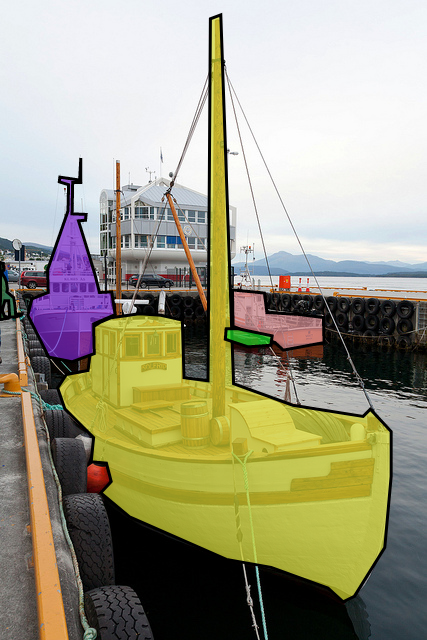
\includegraphics[scale=0.4]{images/coco.png}
    \caption{Example image from the COCO dataset, different objects are segmented at pixel values.}
    \label{fig:coco}
\end{figure}

\subsection{Custom datasets}
\label{sec:cust_dataset}
A big part of this project has been to compile and annotate a dataset of images relevant to this project. This means that images are captured in environments where the algorithm should perform well, this being in areas around Trondheimsfjorden or similar areas.


\begin{table}[h!]
\centering
\begin{tabular}{l|l}
Dataset           & Number of images \\ \hline
Trondheim         & 114              \\
Trondheimsfjorden & 472              \\
Hovik             & 1197             \\
Various           & 133              \\ \hline
Total             & 1916            
\end{tabular}
\end{table}

\newpage

These datasets were then divided into the following datasets

\begin{table}[h!]
\centering
\begin{tabular}{l|l|l|l}
Category                   & Dataset           & Number of images & Category total \\ \hline
                           & Trondheimsfjorden & 472              &                \\
                           & BoatsFar        & 1215             &                \\
Sailing boats              & BoatsClose      & 36               & 1723           \\ \hline
 & MooredBoats  & 108              &             \\
Moored boats and buildings & MooredBoatsHouses  & 108              & 108            \\ \hline
Buildings                  & Houses         & 89               & 89            
\end{tabular}
\caption{In the dataset names houses are used for buildings to let the abbreviation "h" be used for buildings ([h]ouses), since "b" is used for boats later in this work. MooredBoats and MooredBoatsHouses contains the same images, in MooredBoatsHouses the buildings in the dataset are labeled as buildings, in MooredBoats they are not.}
\end{table}

In \citep{Tangstad2017}, the detection algorithm used misclassified buildings as boats, and this issue has also been observed during testing of Yolo and SSD. For this reason, datasets consisting images of buildings were compiled, to be able to verify whether training on these images will reduce these misclassifications. The Trondheimsfjorden dataset has been kept as is, and not split into the other sub-datasets. The reasoning for this is that how the algorithm performs in this environment is an interesting performance metric in this project. 


\vspace{3mm}

All the datasets have been split into test and train directories, where 75 percent of the images are used in training, and 25 percent are employed in testing. This is done randomly, but the same configuration is used in all training and testing to ensure that the detection algorithms have the same preconditions.

\subsubsection{Labeling of Custom Dataset}
\label{sec:labeling}
The custom dataset was annotated using LabelImg \footnote{https://github.com/tzutalin/labelImg}. LabelImg lets the user choose the output format and simplifies the labeling process, also for multiclass-labeling. During labeling the VOC Annotation Guidelines \citep{Everingham2012} have been used, which are:

\begin{outline}
    \1 What to label
       \2 All objects of the defined categories, unless:
        \3 you are unsure what the object is.
        \3 the object is very small (at your discretion).
        \3 less than 10-20\% of the object is visible, such that you cannot be sure what class it is. e.g., if only a tyre is visible it may belong to car or truck so cannot be labeled car, but feet/faces can only belong to a person.
      \2If this is not possible because too many objects, mark the image as bad.
    \1 Viewpoint
       \2 Record the viewpoint of the ‘bulk’ of the object, e.g. the body rather than the head.  Allow viewpoints within 10-20 degrees. If ambiguous, leave as ‘Unspecified.’ Unusually rotated objects, e.g. upside-down people should be left as 'Unspecified.'
    \1 Bounding box
       \2 Mark the bounding box of the visible area of the object (not the estimated total extent of the object).Bounding box should contain all visible pixels, except where the bounding box would have to be made excessively large to include a few additional pixels (less than 5\%) e.g., a car aerial.
    \1 Truncation
       \2 If more than 15-20\% of the object lies outside the bounding box mark as Truncated. The flag indicates that the bounding box does not cover the total extent of the object.
    \1 Occlusion
       \2If more than 5\% of the object is occluded within the bounding box, mark as Occluded. The flag indicates that the object is not visible within the bounding box.
    \1 Image quality/illumination
       \2 Images which are poor quality (e.g., excessive motion blur) should be marked bad.  However, poor illumination (e.g., objects in silhouette) should not count as poor quality unless objects cannot be recognized. Images made up of multiple images (e.g., collages) should be marked bad.
    \1 Clothing/mud/ snow etc.
       \2 If an object is ‘occluded’ by a close-fitting occluder e.g., clothing, mud, snow, etc., then the occluder should be treated as part of the object.
    \1 Transparency
       \2 Do label objects visible through glass but treat reflections on the glass as occlusion.
    \1 Mirrors
       \2 Do label objects in mirrors.
    \1 Pictures
       \2 Label objects in pictures/posters/signs only if they are photorealistic but not if cartoons, symbols, etc.
\end{outline}

\section{Detection framework}
Object detection using deep learning based methods is a field of research which is rapidly changing, and new algorithms and methods have continously been presented in recent years. When new methods and articles are released to the public, these algorithms have performance data which makes it possible to compare them to already existing algorithms. These statistics are based on the performance of the algorithms on standard datasets, such as COCO \citep{COCO}, VOC Pascal \citep{Everingham2007}, \citep{Everingham2012}, and Imagenet \citep{Imagenet}, and gives an estimate of how fast and how accurate the algorithm is. When trained on these datasets, which include multiple classes, e.g. persons, cars and dogs, they become general purpose object detectors. In other words, object detectors which are trained to handle different objects in different settings. In this project, the object of interest is maritime vessels, and possibly other objects related to navigation and obstacle avoidance. Thus, the focus in this report is a specialized object detector that is trained for detecting the objects mentioned above. The performance statistics from object detection articles can thus only be used as a guideline for how well it will perform as a specialized object detector in a maritime environment. 

\vspace{3mm}

The different, currently existing, object detection algorithms could potentially perform on a vastly different level depending, e.g. on the lighting conditions, how big the object of interest is in the image, and which data they are trained on. Their performance can also significantly differ based on how the algorithm is configured. Yolo, for instance, can perform better on smaller objects by increasing the grid size mentioned in chapter \ref{sec:yolo}. The performance of different detection algorithms in maritime environments based on their configuration and on which data it is trained on, is a landscape that is not explored fully. This project aims to make it possible to more efficiently and systematically navigate in this landscape and to begin a heuristic approach to find directions worth continuing to research.

\begin{figure}[h!]
    \centering
    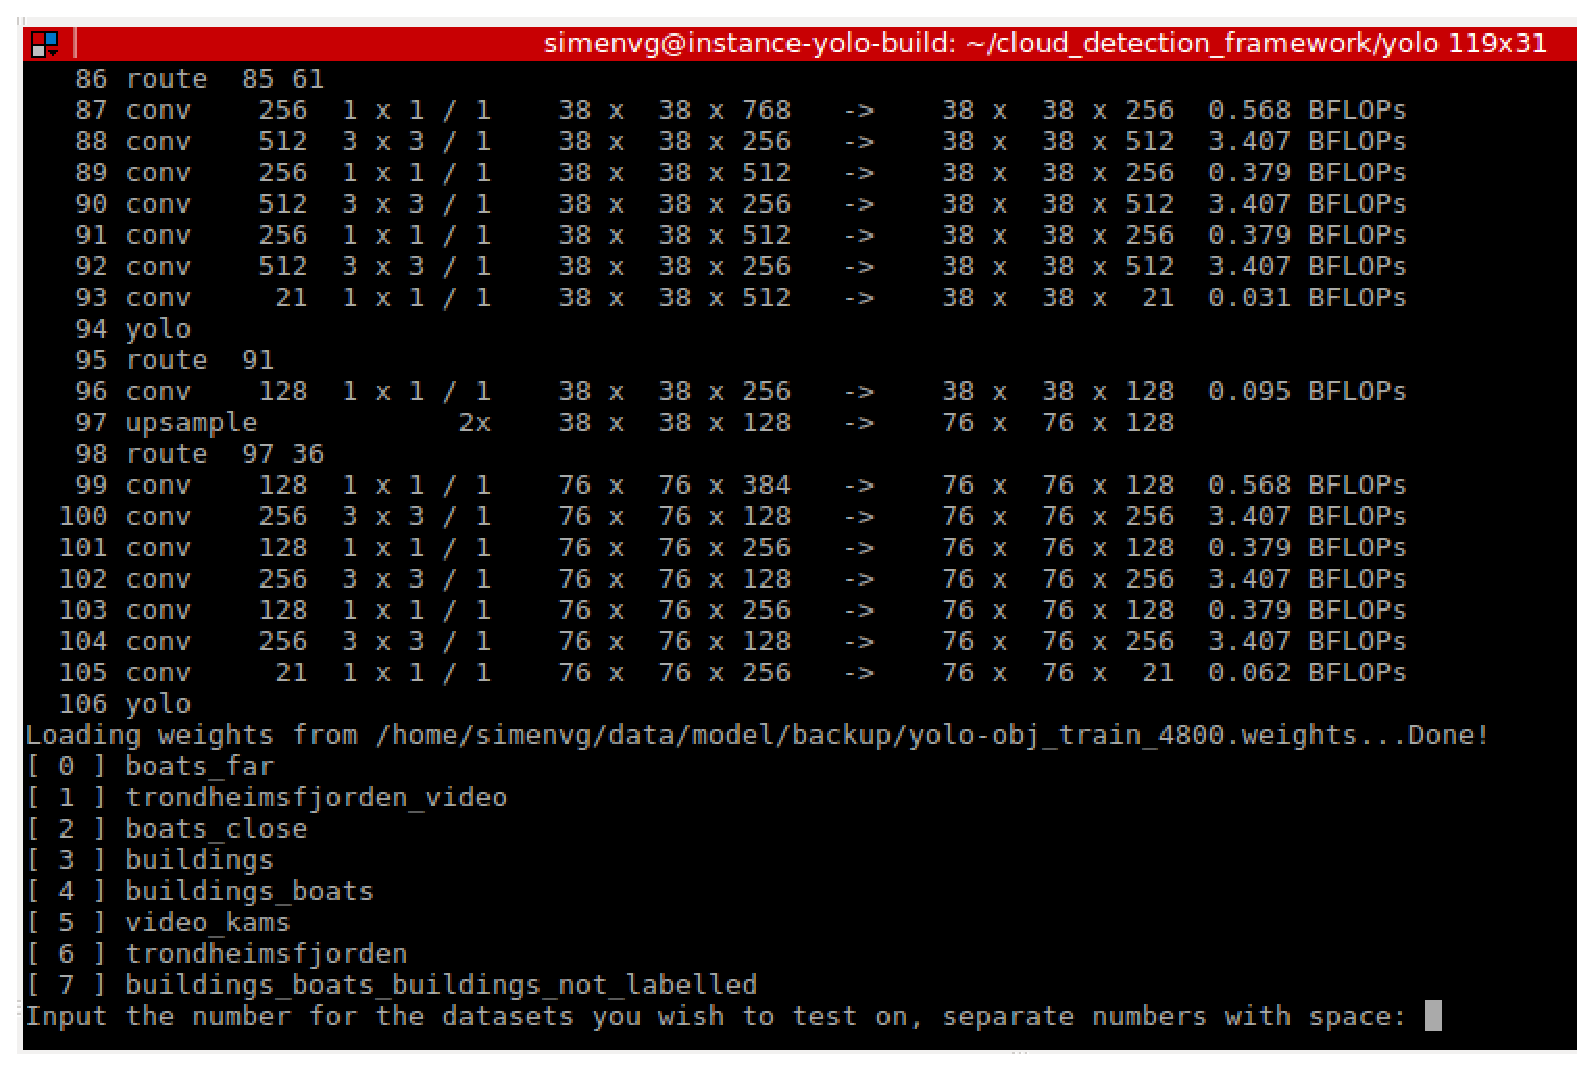
\includegraphics[width=0.8 \textwidth]{images/cloud_detection_pic.eps}
    \caption{Example image from the Cloud Detection Framework, here the user is prompted which datasets to test Yolo on.}
    \label{fig:cloud_det}
\end{figure}

\subsection{Hardware}
One of the first issues one encounters while trying to train a convolutional neural network is the need for specific hardware that has the computational capacity to train and test the network in a reasonable amount of time. All the object detection algorithms mentioned in this thesis are implemented with support for Graphics Processing Unit (GPU) computations. According to Nvidia, GPUs alone increased the computational speed by a factor of 1,000 over a span of 10 years, greatly supporting the progress in deep learning \citep{Dettmers2015}. The most popular library used for GPU processing for neural networks is today CUDA, which is developed by Nvidia. Hence, the GPU needed for more efficient training and testing of neural networks has to be a Nvidia GPU. 

\vspace{3mm}

Another problem that arises when working with the cutting edge detection algorithms is to get an environment set up correctly. Libraries, programs, and drivers have to be installed the correct way, and configuration files and paths must be set accordingly. This may sound trivial, but the road from an annotated dataset to a trained object detector can be long and frustrating. A goal in this project is to make this process as simple as possible, this enables future master students or researchers to focus more on the actual problem and not spend time on creating the system. 

\subsection{Google Cloud}
The solution to the hardware problem in this project is to use a cloud computing service, in this case, Google Cloud. Other cloud computing solutions exist, where some of the most popular are Amazon AWS and Microsoft Azure. Google Cloud was chosen because they give 300\$ in free credit for opening an account, which makes it an economical choice in a testing phase.

\vspace{3mm}

Google Cloud lets you open an instance where you can specify the operating system and hardware according to the requirements of the user. The instance opens on a clean installation of the selected operating system, and an object detection environment can, therefore, be set up the same way for every instance. In this project, the operating system used is Ubuntu 16.04 and the GPU used is a Nvidia Tesla K80. A detailed explanation of how Google Cloud was configured can be seen in Appendix A in chapter \ref{ap_gcloud}.

\vspace{3mm}

It should also be noted that this system work on other cloud computing services, as long as the hardware satisfies the requirements. 

\subsection{Cloud Instance Setup}
The Google Cloud instance can be configured by cloning the Cloud Detection Framework Github repository\footnote{https://github.com/simenvg/cloud\_detection\_framework}. Running the setup.sh file will install and set up the following 

\begin{outline}
    \1 CUDA and cudnn
       \2 Nvidia libraries used to run computations on the GPU. 
    \1 Tensorflow
       \2 Google's software library for dataflow programming
       \2 Tensorflows models directory from GitHub is also downloaded and with it its object detection API
    \1 Yolo
       \2 Yolo's GitHub repository is downloaded, modified to have GPU support and built
    \1 Directory structure
       \2 Directories and subdirectories are made to handle training data input and to have a consistent system configuration for the different object detection algorithms
    \1 Required Python libraries
    \1 Virtual Environments
       \2 A python3 virtual environment is set up to handle compatibility with different frameworks.
\end{outline}



When the setup file has been executed, data can be uploaded to the Google cloud instance. When data have been uploaded, and the Google cloud instance has been set up by running \url{setup.sh}, the system is ready to train.

\subsection{Training Yolo}
In this project Yolov3 is used, the latest version of Yolo at the time of writing. To train Yolo, run the file \url{train_yolo.py}, this will:

\begin{itemize}
    \item Prompt the user and ask which datasets the user wishes to train on.
    \item Set up a model folder where all files needed for testing is saved.
    \item Convert annotation files for the images to Yolo format
    \item Make a train.txt file which contains the path to all the images that are to be used in training
    \item Make configuration files based on the training data needed to run YOLO.
    \item Edit Yolo's main configuration file (.cfg file) to have the correct batch-size, the number of classes, subdivision, and filters, based on the number of classes in the training data and the hardware used on the Google cloud instance.
    \item Load pre-trained weights
    \item Begin training.
\end{itemize}

During training, Yolo will save weights every 400 iterations to the model repository. It will continue training until the user exits the process, or when it reaches 40 000 iterations. When the process runs the average loss will be written to the terminal for every iteration, and training can be stopped when it is sufficiently low. In this project all the detection models were trained for approximately 24 hours.

\newpage

\subsubsection{Pre-trained weights yolo}
Yolo comes with the following pre-trained weights

\begin{table}[h!]
\begin{tabular}{lllllll}
Model               & Top-1 & Top-5 & Ops      & GPU     & CPU    & Weights \\ \hline
AlexNet             & 57.0  & 80.3  & 2.27 Bn  & 3.1 ms  & 0.29 s & 238 MB  \\
Darknet Reference   & 61.1  & 83.0  & 0.96 Bn  & 2.9 ms  & 0.14 s & 28 MB   \\
VGG-16              & 70.5  & 90.0  & 30.94 Bn & 9.4 ms  & 4.36 s & 528 MB  \\
Extraction          & 72.5  & 90.8  & 8.52 Bn  & 4.8 ms  & 0.97 s & 90 MB   \\
Darknet19           & 72.9  & 91.2  & 7.29 Bn  & 6.2 ms  & 0.87 s & 80 MB   \\
Darknet19 448x448   & 76.4  & 93.5  & 22.33 Bn & 11.0 ms & 2.96 s & 80 MB   \\
Resnet 18           & 70.7  & 89.9  & 4.69 Bn  & 4.6 ms  & 0.57 s & 44 MB   \\
Resnet 34           & 72.4  & 91.1  & 9.52 Bn  & 7.1 ms  & 1.11 s & 83 MB   \\
Resnet 50           & 75.8  & 92.9  & 9.74 Bn  & 11.4 ms & 1.13 s & 87 MB   \\
Resnet 101          & 77.1  & 93.7  & 19.70 Bn & 20.0 ms & 2.23 s & 160 MB  \\
Resnet 152          & 77.6  & 93.8  & 29.39 Bn & 28.6 ms & 3.31 s & 220 MB  \\
ResNeXt 50          & 77.8  & 94.2  & 10.11 Bn & 24.2 ms & 1.20 s & 220 MB  \\
ResNeXt 101 (32x4d) & 77.7  & 94.1  & 18.92 Bn & 58.7 ms & 2.24 s & 159 MB  \\
ResNeXt 152 (32x4d) & 77.6  & 94.1  & 28.20 Bn & 73.8 ms & 3.31 s & 217 MB  \\
Densenet 201        & 77.0  & 93.7  & 10.85 Bn & 32.6 ms & 1.38 s & 66 MB   \\
Darknet53           & 77.2  & 93.8  & 18.57 Bn & 13.7 ms & 2.11 s & 159 MB  \\
\textbf{Darknet53 448x448}   & \textbf{78.5}  & \textbf{94.7}  & \textbf{56.87 Bn} & \textbf{26.3 ms} & \textbf{7.21 s} & \textbf{159 MB} 
\end{tabular}
\caption{Pre-trained weights Yolo}
\label{yolo_tab}
\end{table}

Table \ref{yolo_tab} is from \citep{YOLOv3}. These models are trained on ImageNet, and the top-1 and top-5 columns show the accuracy of the pre-trained model on the ImageNet dataset. In this project, the Darknet53 448x448 model has been used. 



\newpage

\subsection{Training SSD}
In this project Tensorflows implementation of SSD Mobilenet is used. To train SSD run the file \url{train_ssd.py}, this will:

\begin{itemize}
    \item Prompt the user and ask which datasets the user wishes to train on
    \item Convert annotations and images to tfrecords\footnote{Tfrecords are Tensorflows binary file format. Binary files uses less storage and are beneficial when working with large datasets.}, which Tensorflow needs to train.
    \item Update SSD's configuration file with correct paths to training data, classes, and filters.
    \item Load pre-trained weights
    \item Begin training
\end{itemize}

\url{train_ssd.py} will also save all files needed for testing to the model directory. It will save the weights based on time, and not based on iterations like Yolo. At what iteration the happens depends on the size of the dataset and the hardware used. 

\subsubsection{Pre-trained weights SSD}
SSD is implemented using Tensorflow's object detection API. Tensorflow offers several detection algorithms shown in table \ref{ssd_tab}. These are trained on the Coco dataset and comes with different configurations. The cloud detection framework is designed to be able to implement other detection algorithms easily. The SSD version chosen in this project is ssd\_mobilenet\_v1\_coco. The Cloud Detection Framework is designed such that to implement any of the other models shown in figure \ref{ssd_tab} one only needs to download another model and edit a few lines in a configuration file. The models implemented in Tensorflow's object detection API is also rapidly expanding. In the summer of 2017, there were eight models available, in December of 2018, there are 25. This means that by using the Cloud Detection Framework one can easily train and test new, cutting-edge models that Google supply through Tensorflow.

\begin{table}[h!]
\begin{tabular}{lll}
Model name                                                      & Speed (ms)  & COCO mAP{[}\textasciicircum{}1{]} \\ \hline
\textbf{ssd\_mobilenet\_v1\_coco}                               & \textbf{30} & \textbf{21}                       \\
ssd\_mobilenet\_v1\_0.75\_depth\_coco ☆                         & 26          & 18                                \\
ssd\_mobilenet\_v1\_quantized\_coco ☆                           & 29          & 18                                \\
ssd\_mobilenet\_v1\_0.75\_depth\_quantized\_coco ☆              & 29          & 16                                \\
ssd\_mobilenet\_v1\_ppn\_coco ☆                                 & 26          & 20                                \\
ssd\_mobilenet\_v1\_fpn\_coco ☆                                 & 56          & 32                                \\
ssd\_resnet\_50\_fpn\_coco ☆                                    & 76          & 35                                \\
ssd\_mobilenet\_v2\_coco                                        & 31          & 22                                \\
ssd\_mobilenet\_v2\_quantized\_coco                             & 29          & 22                                \\
ssdlite\_mobilenet\_v2\_coco                                    & 27          & 22                                \\
ssd\_inception\_v2\_coco                                        & 42          & 24                                \\
faster\_rcnn\_inception\_v2\_coco                               & 58          & 28                                \\
faster\_rcnn\_resnet50\_coco                                    & 89          & 30                                \\
faster\_rcnn\_resnet50\_lowproposals\_coco                      & 64          &                                   \\
rfcn\_resnet101\_coco                                           & 92          & 30                                \\
faster\_rcnn\_resnet101\_coco                                   & 106         & 32                                \\
faster\_rcnn\_resnet101\_lowproposals\_coco                     & 82          &                                   \\
faster\_rcnn\_inception\_resnet\_v2\_atrous\_coco               & 620         & 37                                \\
faster\_rcnn\_inception\_resnet\_v2\_atrous\_lowproposals\_coco & 241         &                                   \\
faster\_rcnn\_nas                                               & 1833        & 43                                \\
faster\_rcnn\_nas\_lowproposals\_coco                           & 540         &                                   \\
mask\_rcnn\_inception\_resnet\_v2\_atrous\_coco                 & 771         & 36                                \\
mask\_rcnn\_inception\_v2\_coco                                 & 79          & 25                                \\
mask\_rcnn\_resnet101\_atrous\_coco                             & 470         & 33                                \\
mask\_rcnn\_resnet50\_atrous\_coco                              & 343         & 29                               
\end{tabular}
\caption{Pre-trained models SSD}
\label{ssd_tab}
\end{table}


\newpage

\subsection{Testing with Cloud Detection Framework}
During testing of the detection algorithms, a problem arose when testing on large datasets. When testing on hundreds of images containing several objects the data could not be saved in JSON format as a txt-file due to heavy memory requirements. Thus, a different solution was implemented where detections were saved in a database using SQL. This divides the process of testing into two phases. One where the algorithm is run on the test images and all detections are written to a database. The other phase draws the detections, and the ground truth bounding boxes onto the test images and saves them, and calculates statistics on how well the algorithm performed. These results are saved to the "results" directory.

\vspace{3mm}

Both YOLO and SSD will assume that the model is set up as it is after training. This means that a trained model can be downloaded, and uploaded to new instances in Google Cloud. This makes it easy to reuse trained models, and to continue working on other's research.









\cleardoublepage